\section{Le client}
\label{sec:customer}

\begin{wrapfigure}{L}{0.35\textwidth}
    \centering
    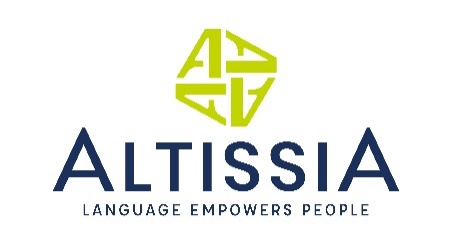
\includegraphics[width=0.35\textwidth]{altissia-logo.jpeg}
\end{wrapfigure}

Altissia\fnmark est spécialisé dans la création, la mise en œuvre et la réussite de projets linguistiques personnalisés et contextualisés pour le monde éducatif, professionnel et institutionnel.  
Son siège social est basé sur le campus de Louvain-La-Neuve (Belgique).
Son activité et sa présence structurelle s’étendent dans le monde (France, Espagne, Italie, Maroc, Indonésie, Singapour, Pérou, Brésil et Canada) avec une centaine de collaborateurs.
\begin{wrapfigure}{R}{0.4\textwidth}
    \centering
    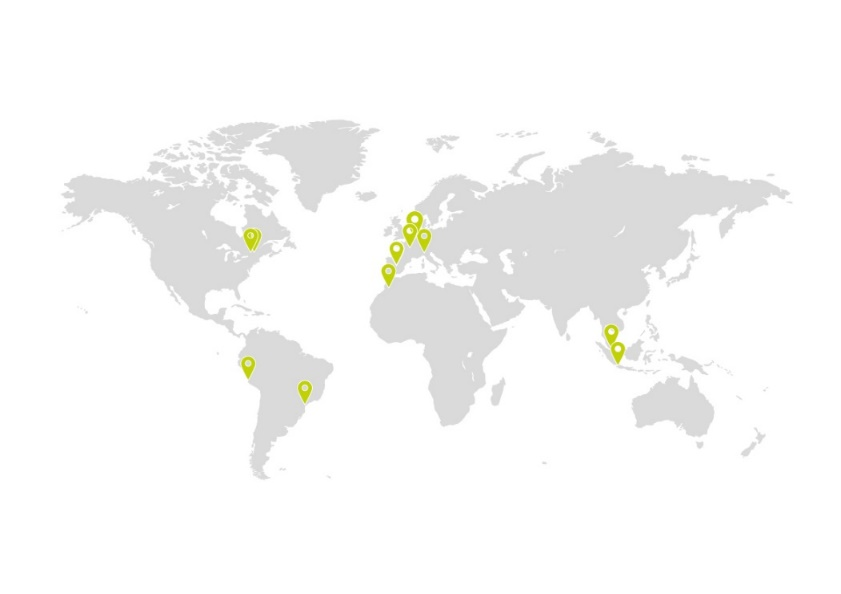
\includegraphics[width=0.4\textwidth]{altissia-presence-map.jpeg}
\end{wrapfigure}

\fntext{Merci à Altissia pour avoir fourni le texte et les images constituant cette section \ref{sec:customer} à l'exception de la sous-section \ref{ssec:target-service}.}

\subsection{Panorema des offres et services}
\paragraph{}
Altissia s’est assigné comme mission, l’accès au plus grand nombre possible d’apprenants à l’apprentissage des langues et du langage sous une forme académique, structurante et ludique. Ses maîtres-mots sont la mobilité, l’immersion, la contextualisation, la personnalisation, l’Innovation, la Recherche et le Développement (IRD), la valorisation de la diversité et l’humanisme.

\paragraph{}
La porte d’entrée de tous les projets est une plateforme à la fois contextualisée et personnalisée en fonction de l’autorité contractante et de l’apprenant,
et globale puisque tous les projets englobent une grande variété de moyens,
tant présentiels que mobiles, pour permettre la réussite du projet.

\paragraph{}
Voici les principaux services qui composent les projets d’Altissia :
\begin{itemize}
    \item Une plateforme d’auto-formation, en ligne, dans 22 langues officielles de l’Union européenne
    \item Un outil adaptatif d’évaluation de niveau dans 24 langues
    \item Un service informel d’apprentissage des langues par l’actualité, renouvelé quotidiennement
    \item Le développement de contenus pédagogiques sur mesure
    \item Un réseau social d’échange linguistique
    \item Une solution de remédiation orthographique automatisée
    \item Des dispositifs multiples d’accompagnement de projet et des intervenants, combinant aussi bien les outils distanciels que présentiels.
\end{itemize}
\begin{figure}[ht]
    \centering
    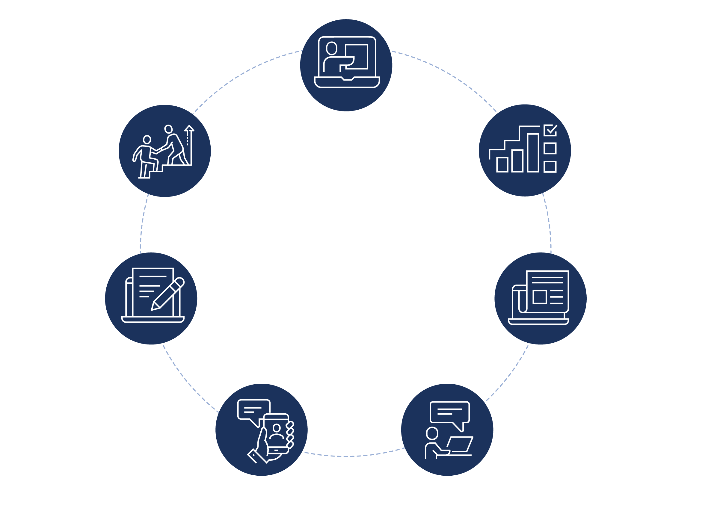
\includegraphics{altissia-services.png}
    \caption{Les multiples services proposés par Altissia}
    \label{fig:altissia-services}
\end{figure}

\subsection{Références}
\paragraph{}
Depuis quinze ans, Altissia œuvre à la mise en place, au déploiement et à la gestion de nombreux projets ambitieux d’évaluation et d’enseignement des langues à distance. Dans les lignes qui suivent, nous présentons quelques-unes des références majeures d’Altissia.

\subsubsection{Erasmus+ OLS}
\begin{wrapfigure}{R}{0.3\textwidth}
    \centering
    
\includegraphics[width=0.3\textwidth]{erasmusplus-logo.png}
\end{wrapfigure}
\paragraph{}
Le projet Erasmus+ OLS (\url{www.erasmusplusols.eu}) a été lancé par la Commission européenne en 2014 pour une période de sept ans. Ce projet consiste à créer, développer et promouvoir deux sous-projets, dans le cadre d’un consortium entre Altissia, le Centre de Langues (CLL\cite{cll_actualites_nodate}) et l’Université catholique de Louvain-la-Neuve (UCL).
 
\paragraph{}
Le premier sous-projet consiste à élaborer une plateforme de test de 24 langues pour tous les participants. Ce projet politique a pour mission de tester les participants au départ et au retour de leur séjour académique (de 1 à 12 mois) dans un établissement de l’un des pays de l’Union européenne.

\paragraph{}
Le second sous-projet consiste à élaborer, maintenir et promouvoir une plateforme d’apprentissage de 22 langues européennes. Cette plateforme doit permettre à l’apprenant d’améliorer toutes ses compétences linguistiques, par le biais de différentes activités, telles que des MOOC, des actualités internationales pédagogisées, des cours de groupe en visioconférence, etc.

\paragraph{}
Sur les sept années du projet, le nombre d’apprenants total est estimé à environ 4,5 millions.

\subsubsection{CNED}
\begin{wrapfigure}{R}{0.3\textwidth}
    \centering
    
\includegraphics[width=0.3\textwidth]{cned-logo.png}
\end{wrapfigure}
\paragraph{}
Le Centre national d’enseignement à distance, placé sous la tutelle du ministère de l’Éducation nationale fait confiance à Altissia depuis novembre 2014 pour la mise à disposition de contenus e-learning en anglais, espagnol, allemand, italien, néerlandais et français langue étrangère (FLE) pour les niveaux A1 à C1.

\paragraph{}
Les contenus proposés par Altissia sont intégrés au dispositif \#jeveuxparler, ainsi qu’aux parcours de plusieurs dizaines de filières BTS, conformes aux exigences des programmes officiels de ceux-ci. 

\subsubsection{Wallangues}
\begin{wrapfigure}{R}{0.3\textwidth}
    \centering
    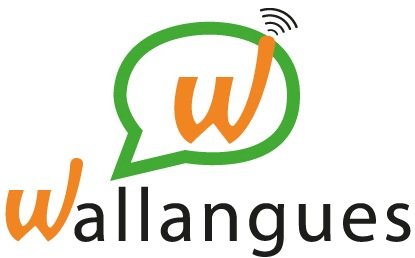
\includegraphics[width=0.3\textwidth]{images/wallangues-logo.jpeg}
\end{wrapfigure}
\paragraph{}
Wallangues (\url{www.wallangues.be}) a été lancé par la Région wallonne (Belgique) en 2011 pour une durée de quatre ans. Ce projet a pour but de donner un accès gratuit à tous les résidents wallons à l’apprentissage des trois langues nationales ainsi qu’à l’anglais. La mission de ce projet est d’améliorer la connaissance des langues pour renforcer la cohésion nationale, permettre un meilleur accès à l’emploi et à la mobilité et permettre une meilleure connaissance « de l’autre » et le respect de chacun.

\paragraph{}
Le public cible est d’environ 2,8 millions d’habitants. Ce projet a d’ailleurs été désigné par les citoyens comme la meilleure initiative du gouvernement wallon et, en 2015, le projet a été renouvelé pour cinq années supplémentaires, jusqu’en 2020. Une des particularités de ce projet est la collaboration et le partenariat inclusif entre le projet et les institutions publiques, telles que les ministères de l’Emploi et de la Formation continue et toutes les organisations semi-publiques en lien avec la jeunesse, l’emploi, les nouvelles technologies, l’alphabétisation et les ASBL (Associations sans but lucratif). L’ensemble des acteurs associés au projet partagent des missions qui ont un lien avec l’éducation, la formation, l’inclusion, l’intégration sociale, le sport et la culture.

\subsubsection{Mogilinguas - Mogi Das Cruzes -- Sao Paulo}
\begin{wrapfigure}{R}{0.3\textwidth}
    \centering
    
\includegraphics[width=0.3\textwidth]{mogi-linguas-logo.png}
\end{wrapfigure}
\paragraph{}
Mogilinguas (\url{www.mogilinguas.com.br}) est un projet qui a été lancé en 2017 par la préfecture de la ville de Mogi das Cruzes (Brésil) pour une durée de quatre ans. Ce projet a pour but de donner un accès gratuit à tous les résidents de la ville de Mogi das Cruzes à l’apprentissage de l’espagnol, de l’anglais et du français. 

\paragraph{}
Il s’agit d’un projet multifacette qui consiste à changer le paradigme de l’apprentissage au Brésil et à le mettre à disposition de tous les habitants. De multiples activités sont créées pour rendre le projet citoyen et pour que tous les habitants se l’approprient. Par exemple, une antenne Mogilinguas est installée dans la ville avec des points de rencontre itinérants. 

\paragraph{}
Le nombre de participants concernés est d’environ 420 000. 

\subsubsection{Des entreprises}
\begin{figure}[ht]
    \centering
    
\includegraphics[width=0.1\textwidth]{images/companies/ing-logo.jpeg}
    
\includegraphics[width=0.1\textwidth]{images/companies/swift-logo.jpeg}
    
\includegraphics[width=0.1\textwidth]{images/companies/total-logo.jpeg}
    
\includegraphics[width=0.1\textwidth]{images/companies/carrefour-logo.jpeg}
    
\includegraphics[width=0.1\textwidth]{images/companies/microsoft-logo.png}
    
\includegraphics[width=0.1\textwidth]{images/companies/belgacom-logo.jpeg}
    
\includegraphics[width=0.1\textwidth]{images/companies/ubisoft-logo.jpeg}
    
\includegraphics[width=0.1\textwidth]{images/companies/caterpillar-logo.jpeg}
    
\includegraphics[width=0.1\textwidth]{images/companies/solvay-logo.jpeg}
    
\includegraphics[width=0.1\textwidth]{images/companies/accenture-logo.jpeg}
    
\includegraphics[width=0.1\textwidth]{images/companies/dhl-logo.jpeg}
    
\includegraphics[width=0.1\textwidth]{images/companies/bpost-logo.jpeg}
    \caption{Quelques unes des entreprises qui ont choisi Altissia}
    \label{fig:companies-logo}
\end{figure}
Altissia compte parmi ses clients des entreprises de renoms telles que ING, Swift, Baxter, Total, Carrefour, Microsoft, Ubisoft, Proximus, Caterpillar, Solvay, Accenture, DHL, Bpost, etc.

\subsubsection{Éducation}
\begin{figure}[ht]
    \centering
    
\includegraphics[width=0.1\textwidth]{images/education/u-antwerpen-logo.jpeg}
    
\includegraphics[width=0.1\textwidth]{images/education/ucl-logo.jpeg}
    
\includegraphics[width=0.1\textwidth]{images/education/cll-logo.jpeg}
    
\includegraphics[width=0.1\textwidth]{images/education/u-st-louis-logo.jpeg}
    
\includegraphics[width=0.1\textwidth]{images/education/ichec-logo.png}
    
\includegraphics[width=0.1\textwidth]{images/education/ephec-logo.jpeg}
    
\includegraphics[width=0.1\textwidth]{images/education/uppna-logo.png}
    \caption{Quelques acteurs de l'éducation que Altissia aide dans leur mission}
    \label{fig:educations-logo}
\end{figure}
Altissia sert aussi des acteurs dans l'éducation tels que ICHEC, CLL, UCL, EPHEC, Upna, Universiteit Antwerpen, Université Saint-Louis, etc.

\subsection{Concurrents}
Altissia propose une offre complète et variée. Son offre se décline en plusieurs langues, est disponible sur plusieurs plateformes, prends diverses formes et occupe toutes les facettes du marchés (B2B, B2I, B2E et B2C).
De ce fait, de nombreux concurrents existent mais sur des segments restreints de l'espace qu'occupe Altissia.

Ses concurrents les plus directs sont Rosetta Stone, 7 Speaking, GOFluent, Speexx et Télélangue.

\subsection{Service cible de l'application}
\label{ssec:target-service}
\paragraph{}
L'application sera utilisée par le service linguistique et le service informatique qui sont conjointement responsables du contenu de cours
et du développement des plateformes de cours.
Ces deux services comptabilisent une cinquantaine de personnes et comportent des profils de linguistes, développeurs informatiques,
concepteurs d'interfaces utilisateur, administrateurs systèmes, chefs de projets et analystes fonctionnels.

\paragraph{}
Le personnel IT s'occupera de configurer l'outil tandis que les utilisateurs principaux seront que les linguistes ainsi que le support.
